%!TEX encoding = UTF-8 Unicode

%!TEX root = ../solutions.tex

\ExerciseSolution{\ExeWeekSEVEN}

\Task %Uppgift 1

\Subtask
\begin{REPLnonum}
scala> val pt = (15.9, 28.9)

scala> math.hypot(pt._1, pt._2)
res0: Double = 32.98514817307935
\end{REPLnonum}

\Subtask  \code{val (x, y) = pt}

\Subtask  \code{(String, String, Double, Boolean)}

\Subtask  \code{Vector[(Double, Double)]}

\Subtask  \code{huvudstäder :+ ''Danmark'' -> ''Köpenhamn''}

\Subtask  \code{Vector[Double]}

\Subtask  \code{val antalUdda = (1234 to 3456).map(i => div(i, 2)._2).sum}

\Subtask  0-tupel

\Task %Uppgift 2

\Subtask  \code{mittKonto.saldo = (math.random * 1000000).toInt}

\Subtask  Går ej eftersom val är oföränderlig, man får alltså ett Error.

\Task %Uppgift 3

\Subtask  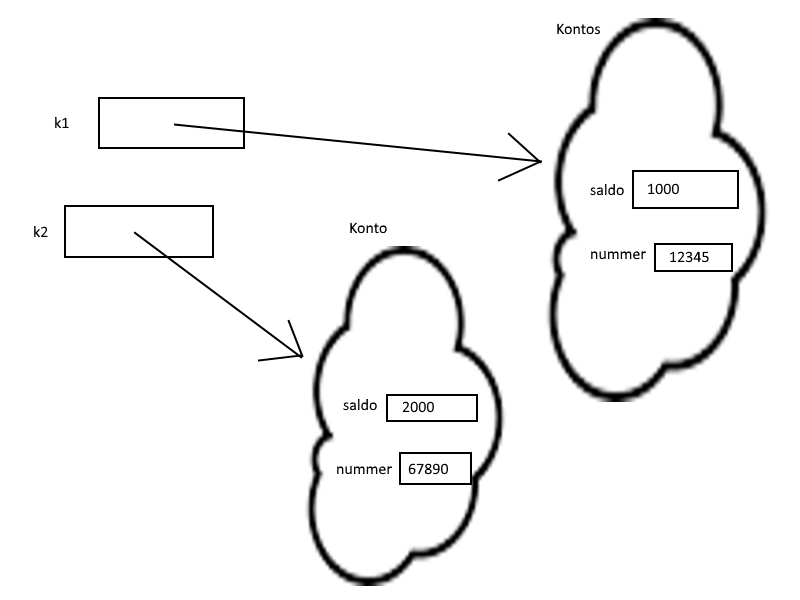
\includegraphics[scale=0.5]{../img/w04-solutions/uppgift-3a}

\Subtask
Tilldelningen på rad 8 \code{k1.nummer = 12345L} ger felmeddelande eftersom variablen är oföränderlig.

\Task %Uppgift 4

\Subtask  \code{String = Konto@cd576}, där \code{Konto@cd576} är ett unikt namn som identifierar instansen.

\Subtask  Ja.

\Subtask
\begin{REPLnonum}
scala> k.saldo = 42
scala> k2.saldo = 67
\end{REPLnonum}

\Subtask  Eftersom variablen är oföränderlig ges ett felmeddelande.

\Subtask  En fördel med klass är att man kan specificera att variablen ska kunna vara föränderlig. En till är att man kan inkludera metoder i klassen som man vill kunna använda på värdena.

\Task %Uppgift 5

\Subtask
Det går bra att ändra på variablen saldo i instansen av Konto1 men inte av Konto2 där man får ett error på raden ''k2.saldo += 1000''

\Subtask -

\Subtask
''println(k.saldo)'' och ''k.saldo += 1000'' ger båda error, pga privat attribut.

\Subtask
\begin{Code}
def ut(belopp: Int): (Int, Int) = {
	if(saldo >= belopp) {
		saldo -= belopp
		(belopp, saldo)
	} else {
		val temp = saldo
		saldo = 0
		(temp, 0)
	}
}
\end{Code}

\Subtask
Lägg till en if-sats i båda funktionerna som omsluter den gamla koden.
\begin{Code}
def ut(belopp: Int): (Int, Int) = {
  if(belopp >= 0) {
    if(saldo >= belopp) {
      saldo -= belopp
      (belopp, saldo)
    } else {
      val temp = saldo
      saldo = 0
      (temp, 0)
    }
  }
}

def in(belopp: Int): Unit = {
  if(belopp >= 0) {
    saldo += belopp
  }
}
\end{Code}

\Subtask
Genom att göra attributet privat och gör egna metoder kan man se till att attriuten endast ändras på säkra sätt. Så inte fel uppstår.

\Task %Uppgift 6

\Subtask
''val i: Int = pt.x'' error: type mismatch;
Eftersom typen Int ej är kompatibel med ett värde av typen Double.

''val p: Double = new Punkt(5.0, 5.0)'' error: type mismatch;
Eftersom typen Double ej är kompatibel med ett värde av typen Punkt.

''val p = new Punkt(5.0, 5.0): Double'' error: type mismatch;
Eftersom typen Double ej är kompatibel med ett värde av typen Punkt.

\Subtask
Rad 3 till 7 i respektive ordning: true, false, false, true och false.

\Task %Uppgift 7
\\Definierar klassen Punkt.
\\En variabel med namnet pt skapas med typen Punkt.\
\\true
\\true
\\String = 1.0
\\skriver ut: 1.0
\\En variabel med namnet a skapas med typen Any.
\\error: value x is not a member of Any
\\a ges nu typen String
\\String = 2.0
\\error: value y is not a member of Any

\Task %Uppgift 8

\Subtask
''println(pt)'' kallar på pt.toString, och eftersom metoden är överskriven kallas den nya version.

\Subtask  \code{override def toString: String = ''Punkt('' + x + '', '' + y + '').''}

\Subtask
error: overriding method toString in class Object of type ()String;

\Task %Uppgift 9

\Subtask
\begin{REPL}
scala> val pt = Pt(1.0, 2.0)
pt: Pt = Pt(x=1.0,y=2.0)

scala> Pt(4.0, 2.0)
res0: Pt = Pt(x=4.0,y=2.0)

scala> Pt(6.0, 3.0)
res1: Pt = Pt(x=6.0,y=3.0)

scala> Pt(666.0, 1337.0)
res2: Pt = Pt(x=666.0,y=1337.0)
\end{REPL}

\Subtask \code{def apply(): Pt = new Pt(0, 0)}

\Subtask \code{class Rational(val nom: Int, val denom: Int)}

\Subtask
\begin{REPLnonum}
object Rational {
def apply(nom: Int, denom: Int): Rational = new Rational(nom, denom)
}
\end{REPLnonum}

\Subtask
\begin{REPL}
scala> Rational(2, 5)
scala> Rational(2, 7)
scala> Rational(7, 4)
scala> Rational(666, 1337)
\end{REPL}

\Task %Uppgift 10
\Subtask \code{case class Rational(nom: Int, denom: Int)}

\Task %Uppgift 11

\Subtask
\begin{REPLnonum}
scala> Point(3, 4).distToOrigin
res0: Double = 5.0
\end{REPLnonum}

\Subtask
p3.x = 8
p3.y = 10

\Task %Uppgift 12

\Subtask
\\Operatornotation:	4, 6, 10, 12
\\Punktnotation:		3, 5, 8, 9, 11, 13
\\Felmeddelande:		9

\Subtask
\begin{Code}
case class Point(x: Double, y: Double) {
  def distToOrigin: Double = math.hypot(x, y)
  def add(p: Point): Point = Point(x + p.x, y + p.y)
  def +(p: Point): Point = add(p)
  def sub(p: Point): Point = Point(x - p.x, y - p.y)
  def -(p: Point): Point = sub(p)
}
\end{Code}
\begin{REPL}
scala> val p1: Point = Point(1, 9)
scala> val p2: Point = Point(9, 6)
scala> p1.sub(p2)
scala> p1.-(p2)
scala> p2 sub p1
scala> p2 - p2
scala> p1.add(p2.sub(p1))
scala> p1 + (p2 - p1)
\end{REPL}

\Subtask
\begin{Code}
case class Point(x: Double, y: Double) {
  def distToOrigin: Double = math.hypot(x, y)
  def add(p: Point): Point = Point(x + p.x, y + p.y)
  def +(p: Point): Point = add(p)
  def sub(p: Point): Point = Point(x - p.x, y - p.y)
  def -(p: Point): Point = sub(p)
  def scale(a: Double, b: Double) = Point(x * a, y * b)
}
\end{Code}
\begin{REPL}
scala> val p: Point(13,  37)
scala> p.scale(4, 2)
scala> p scale (3, 7)
\end{REPL}

\Task %Uppgift 13

\Subtask  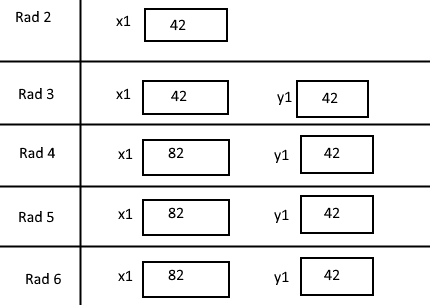
\includegraphics[scale=0.5]{../img/w04-solutions/uppgift-13a}

\Subtask
\begin{enumerate}
\item 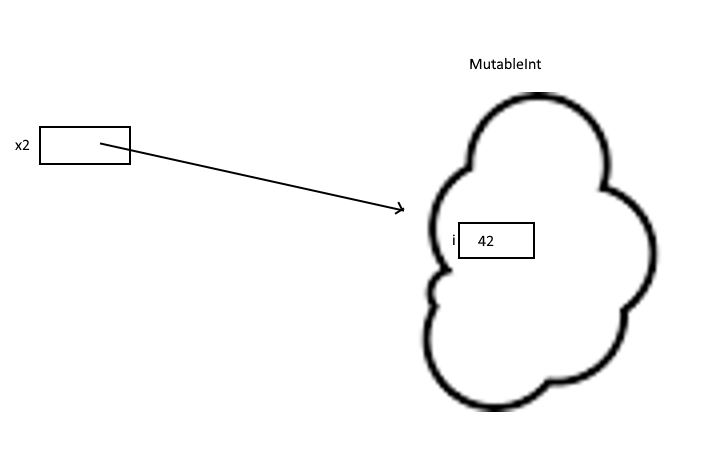
\includegraphics[scale=0.5]{../img/w04-solutions/uppgift-13b-1}
\item 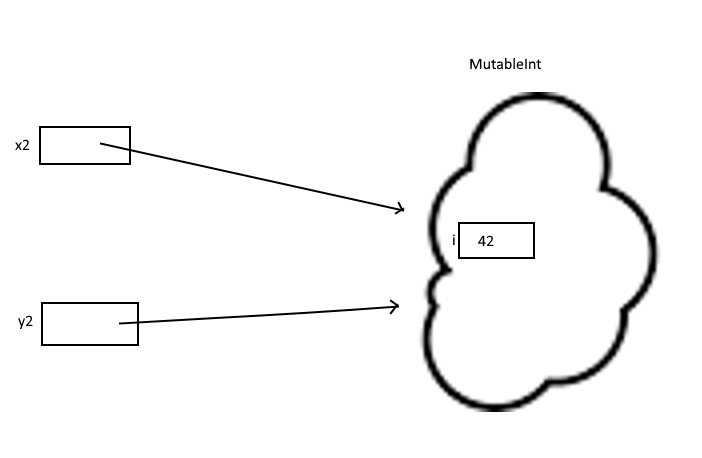
\includegraphics[scale=0.5]{../img/w04-solutions/uppgift-13b-2}
\item 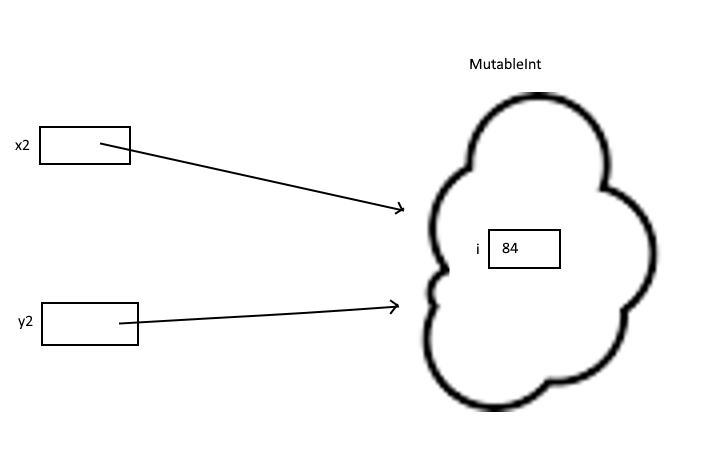
\includegraphics[scale=0.5]{../img/w04-solutions/uppgift-13b-3}
\end{enumerate}

\Subtask
\begin{enumerate}
\item 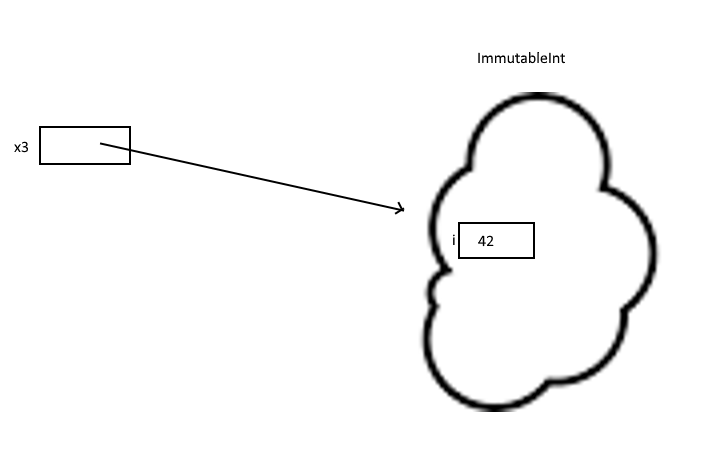
\includegraphics[scale=0.5]{../img/w04-solutions/uppgift-13c-1}
\item 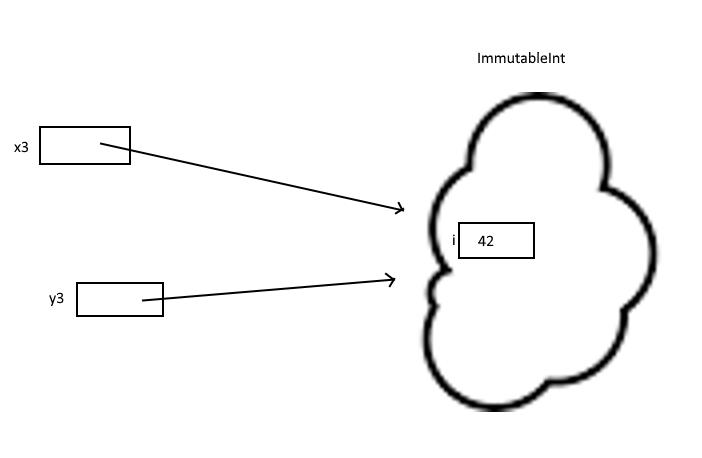
\includegraphics[scale=0.5]{../img/w04-solutions/uppgift-13c-2}
\item 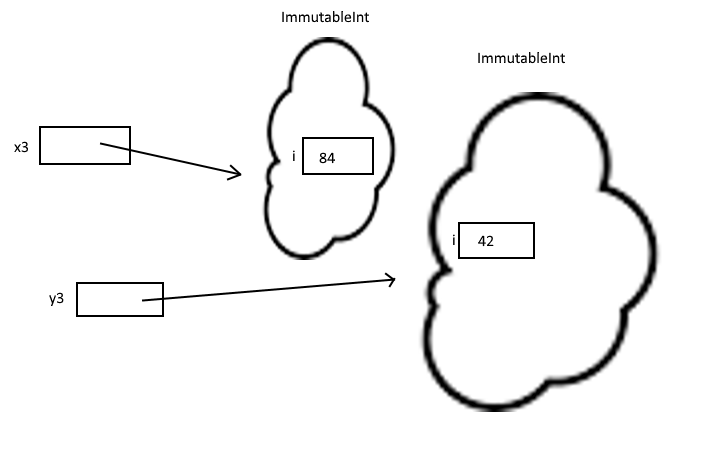
\includegraphics[scale=0.5]{../img/w04-solutions/uppgift-13c-3}
\end{enumerate}

\Subtask  En stor fördel är att vi till exempel kan skicka med en immutable som argument till en metod och vara säkra på att metoden inte ändrar på värdet.

\Task %Uppgift 14

\Subtask  Ungefär 150 metoder.

\Subtask  Ungefär lika många.

\Task %Uppgift 15

\Subtask
\\1. Instansierar en tom vektor med element av typen int och tilldelar värdet till en variabel xs.
\\2. Error eftersom \code{xs :+ ''42''} ger en Vector[Any] när Vector[Int] krävs.
\\3. xs tilldelas ett nytt värde av Vector(43, 64, 46)
\\4. xs skrivs ut.
\\5. Lägger till talet 42 i xs.
\\6. Error: type mismatch
\\7. Skapar en tom Vector i variablen ingenting
\\8. error: type mismatch; found: Int(3), required: Nothing

\Subtask
Tre metoder skapas: den första för att få första elementet i en lista, och eftersom den definieras med specialtypen T går den att använda med alla vektorer oavsett typen av variabeln i vektorn. Den andra får fram sista elementet och den sista hämtar båda två.

En till function definieras längre ner med  namnet ''wrap'', som tar en lista och lägger till ett element längst fram och ett längst bak.

\Task %Uppgift 16

\Subtask  String = ''ka2''

\Subtask  String = ''abra''

\Subtask  false

\Subtask  false

\Subtask  100000

\Subtask  100000

\Subtask  minsta talet i listan

\Subtask  största talet i listan

\Subtask  1

\Subtask  3

\Subtask  Vektor b fast med ''först'' som första element

\Subtask  Vektor a fast med ''sist'' som sista element.

\Subtask  plats 3 i vektorn xs får värdet 42

\Subtask  En ny vektor fylld med ''!'' från och med plats 4 till 10. Men de andra värdena samma som i a.

\Subtask  b sorterad i bokstavsordning

\Subtask  b baklänges

\Subtask  true

\Subtask  true

\Subtask  en vektor med alla unika element i b.

\Task %Uppgift 17

\Subtask
Metoden ger tillbaka en ny Vector[String] som nu består av alla element i a plus alla element i b. I samma ordning med elementen i a först.

\Subtask
Samma som i uppgift a fast vektorn som returnas är av typen Vector[Any]. Det är eftersom Any är den närmsta typen som String och Double delar. Elementen från vektor a är fortfarande först och uppföljt av elementen i stor.

\Subtask
Variablen ys får värdet av en Vector[Int] som innehåller alla talen från xs fast multiplicerade med 5. Alltså ys = 5, 10, 15..., osv.

\Subtask
Functionen tar alla värden från en Vektor och sätter in i ett Set (mängd). Eftersom en mängd ej har dubletter så försvinner ett ''sala'' och ett ''bim'', Vector[String] som returneras blir därför (''sim'', ''sala'', ''bim'').

\Subtask
Metoden head ger första elementet i en samling, och last sista. Därför blir kombinationen av a.head och b.last en ny Vector[String] som består av a:s första element, och b:s första element.

\Subtask
Ger en Vector[String] som innehåller alla element efter det första. Alltså i detta fallet ''ka'' och ''dabra''.

\Subtask
True, eftersom head ger första elementet och tail ger resten, sedan sätter metoden +: ihop dem till en vektor med samma värden som a.

\Subtask
Eftersom ++ sätter ihop alla värden från två vektorer måste vi först omvandla från en sträng till vektor. Resultatet blir en ny vektor av samma typ som innan med a:s första element och b:S sista.

\Subtask
Samma resultat som i h, metoden take börjar från vänster och tar så många element som man skickar med som parameter och gör till en ny lista. Med 1 som parameter motsvarar det att göra Vector(a.head). Metoden takeRight gör samma sak fast från höger.

\Subtask
Metoden drop är motsvarigheten till take fast exkluderar de specifierade elementen istället för att inkludera dem i vektorn.

\Subtask
Eftersom a endast innehåller 3 element returnerar drop(100) en tom vektor.

\Subtask
Returnerar en tom vektor med element typen String

\Subtask
returnerar Vector(true, false)

\Subtask
True, metoden contains kollar om en samling innehåller ett specifikt element.

\Subtask
True. Eftersom en sträng även kan ses som Vector[Char].

\Subtask
Filtrerar vektorn a till att endast innehålla strängar som innehåller k.

\Subtask
Exakt samma som i p

\Subtask
map(\_.toUpperCase) omvandlar alla strängar i a till stora bokstäver
filterNot(\_.contains(''K'')) tar resultatet vi precis fick och tar bort alla strängar som innehåller stora K.

\Subtask
filtrerar så att endast jämna tal finns kvar.

\Subtask
Exakt samma som i s



\Task %Uppgift 18

\Subtask
Vi instansierar en vektor xs med talen 1, 2 och 3.
sedan definierar vi en metod blandat som ger oss en randomiserad version av xs.
sedan definierar vi en till metod som testar om xs är lika med resultatet från blandat. Om det är så returnerar den strängen ''lika'' annars ''olika''.
Sist kör vi en for-loop där vi 100 gånger kör testet, samtidigt räknas hur många gånger ''lika'' returneras.

Vårt resultat är en siffra på hur många gånger xs var samma som en blandad version av sig själv, eftersom det finns 6 permutationer med 3 variabler så borde det vara ungefär 1/6 chans.

\Subtask -

\Subtask
\\ \code{map(\_.trim)} tar bort alla onödiga mellanrum i början och slutet på varje rad
\\ \code{filterNot(\_.startsWith(''<''))} filtrerar bort alla rader som börjar med strängen ''<''
\\ \code{filterNot(\_.isEmpty)} filtrerar bort alla tomma rader.
\\ \code{foreach(println)} skriver ut alla rader.

\Task %Uppgift 19

\Subtask
I princip alla metoder delas, en lista har några fler t. ex. ''::'', '':::'', ''mapConserve'' osv.

\Subtask
Först skapas en lista med 4 sträng värden och instansierar variablen xs med det värdet.
sedan skapar vi en ny lista, som består av ''zero'' + den gamla listan och ger värdet till xs.
Sist instansierar vi en ny variabel ys, som får värdet av xs omvänd plus xs.

\Task %Uppgift 20

\Subtask
true, Boolean

\Subtask
En samling av alla värden i s och t, Set[String]

\Subtask
true, Boolean

\Subtask
false, Boolean

\Subtask
false, Boolean

\Subtask
false, Boolean

\Subtask
true, Boolean

\Subtask
Samlingen s utan elementet ''Stockholm'', Set[String]

\Subtask
Samlingen t utan elementen ''Norge'' och ''Danmark'', Set[String]

\Subtask
returnerar s, Set[String]

\Subtask
Samlingen s utan ''Malmö'' och ''Oslo'', Set[String]

\Subtask
Set(2, 3), Set[Int]

\Subtask
se deluppgift l

\Subtask
Set(1, 2, 3 ,4), Set[Int]

\Subtask
se deluppgift n

\Task %Uppgift 21

\Subtask
Returnerar strängen ''Malmö'' eftersom det värdet är indexerat på platsen ''Skåne''.

\Subtask
Returnerar strängen ''Stockholm'' eftersom det värdet är indexerat på platsen ''Sverige''.

\Subtask
true, eftersom huvudstad innehåller indexet ''Skåne''

\Subtask
false, eftersom huvudstad ej innehåller indexet ''Malmö''. Notera att det är index och inte värden vi
kollar om det finns.

\Subtask
Lägger till indexet ''Danmark'' med värdet ''Köpenhamn'' i samlingen.

\Subtask
Skriver ut alla 2-tupler.

\Subtask
Returnerar ''Oslo'', Note: Om indexet ''Norge'' inte hade funnits hade ''???'' returnerats istället.

\Subtask
Returnerar ''???''

\Subtask
Returnerar en sorterar vektor med alla index.

\Subtask
Returnerar en sorterar vektor med alla värden.

\Subtask
Returnerar en ny mängd men med ''Skåne'' -> ''Malmö'' borttaget.

\Subtask
Returnerar huvudstad mängden eftersom det inte finns ett ''Jylland'' index att ta bort.

\Subtask
Uppdaterar indexet ''Skåne'' till att istället leda till värdet ''Lund''

\Task %Uppgift 22

\Subtask
\begin{REPLnonum}
pairs: scala.collection.immutable.Vector[(String, Long)] =
					Vector((Björn,444), (Maj,441), (Lucy,666))
\end{REPLnonum}

\Subtask
Map[String, Long]

\Subtask
\begin{REPLnonum}
scala> telnr(''Maj'')
res0: Long = 441

scala> telnr.get(''Maj'')
res1: Option[Long] = Some(441)

scala> telnr(''Kim'')
java.util.NoSuchElementException: key not found: 'Kim
  at scala.collection.MapLike$class.default(MapLike.scala:228)
  at scala.collection.AbstractMap.default(Map.scala:59)
  at scala.collection.MapLike$class.apply(MapLike.scala:141)
  at scala.collection.AbstractMap.apply(Map.scala:59)
  ... 32 elided

scala> telnr.get(''Kim'')
res2: Option[Long] = None
\end{REPLnonum}

\Subtask
\begin{REPLnonum}
scala> telnr.getOrElse(''Maj'', -1L)
res0: Long = 441

scala> telnr.getOrElse(''Kim'', -1L)
res1: Long = -1
\end{REPLnonum}

\Subtask
telnr += ''Fröken Ur'' -> 464690510L

\Subtask
telnr.toVector.map(p => p.\_1 -> (''0'' + p.\_2.toString.substring(2)))

\Subtask
Använd metoden toMap och apply.



\Task %Uppgift 23

\Subtask  Metoden maxBy hämtar det element som är ''störst'', på rad två gör \code{x => x._1} att första värdet i tuplerna används för att bestämma vilken som är störst. Likt gör \code{x => x._2} på rad tre att istället det andra värdet används.

\Subtask
\begin{REPLnonum}
scala> xs.maxBy(_._1)
scala> xs.maxBy(_._2)
\end{REPLnonum}

\Subtask
\begin{REPLnonum}
scala> xs.minBy(_._1)
scala> xs.minBy(_._2)
\end{REPLnonum}


\Task %Uppgift 24

Metoden \code{sliding(i: Int).toVector} skapar en ny vector med alla möjliga permutationer av elementen i en vektor med storleken i.
